\documentclass{article}
\title{Theory and Application of MCMC Algorithm on Stochastic Volatility Model}
\author{Yinan Zhu}
\date{}
\usepackage{graphicx}
\usepackage{float}
\begin{document}
\maketitle
\section{Introduction}
The variance of returns of assets tends to change over time. The stochastic volatility model (SV) attempts to model this variance by assuming that they follow some latent stochastic process. It appeared first in the literature of theoretical finance on option pricing, though empirical models are usually described in discrete way. There is evidence the SV models offer increased flexibility over the GARCH family (Geweke(1994)).

However, even the simplest SV model is difficult to fit due to various reasons. Naive strategy of maximum likelihood estimation fails due to the fact that the marginal distribution is evaluated in high dimensional space. Monte Carlo Markov Chain (MCMC), on the other hand, faces difficulty in simulating some non-analytical distributions and people needs to resort to indirect approach such as Metroplis-Hastings algorithm or reject-accept sampling. The topic of this essay will be to analyse the MCMC algorithm for SV model. Instead of general theory, we will focus on a simple SV model where the underling stochastic process is a log-normal autoregressive process. As for the MCMC, we will implement some specific algorithms and test their performance on both artificial and real world data.

The outline of this essay is following. We will introduce the model in section 2.  In section 3, we derive the Bayesian posterior distribution and review three MCMC algorithms to fit the model. In order to compare them quantitatively, in section 4 we held a "competition": We will generate a fake data with underlying model and test which method can recover the hidden parameters. In section 5, we will apply the model on the real world data with these methods and check their results and performance. We gather all the tables and figures at the end.
\section{Basic Model and Notation}
We will focus on a simple form of SV model, which was discussed in many paper, for example Jacquier (1994) and Kim (1998). $y_t$ is the financial series we are interested in, prefiltered to have zero mean. The model is
\[
y_t=\sqrt{h_t}u_t
\]
\[
\ln(h_t)=\alpha+\delta\ln(h_{t-1})+\sigma_\nu\nu_t
\]
\[
u_t,\nu_t\sim N(0,1)
\]
$h_t$ is a latent variable measuring the volatility of $y$, $\delta$ is the volatility persistence. $\sigma_\nu^2$ is the standard deviation of the volatility.

\section{Bayesian Analysis}
\subsection{MCMC}
Assume the prior distribution:
\[
\alpha\sim N(\alpha_0,\sigma_\alpha^2)
\]
\[
\delta\sim N(\delta_0,\sigma_\delta^2)
\]
\[
\sigma_\nu^2\sim IG(\frac{\nu_0}{2},\frac{s_0}{2})
\]
We have the marginal distribution
\begin{eqnarray}
&&p(y,h,\delta,\alpha,\sigma_\nu^2)\propto\frac{1}{\sigma_\nu^{2+\nu_0}}\exp\left(-\frac{(\delta-\delta_0)^2}{2\sigma_\delta^2}-\frac{(\alpha-\alpha_0)^2}{2\sigma_\alpha^2}-\frac{s_0^2}{2\sigma_\nu^2}\right)\nonumber\\
&&\times\prod_{t=2}^{N}\frac{1}{h_t^{\frac{3}{2}}\sigma_\nu}\exp\left(-\frac{y_t^2}{2h_t}-\frac{(\ln h_t-\delta\ln h_{t-1}-\alpha)^2}{2\sigma^2_\nu}\right)
\end{eqnarray}

From which we can derive the posterior distributions are
\[
(\sigma_\nu^2|h,\alpha,\delta)\sim IG\left(\frac{\nu_0+N-1}{2},\frac{s^\prime}{2}\right)
\]
\[
s^\prime=s_0+(N-1)\alpha^2+(1+\delta^2)S_2-\delta^2(\ln h_N)^2-(\ln h_1)^2-2\alpha((1-\delta)S_1-\ln h_1+\delta\ln h_N)-2\delta S_3
\]
\[
(\delta|h,\alpha,\sigma_\nu^2)\sim N\left(\frac{\sigma_\nu^2\delta_0+\sigma_\delta^2(S_3-\alpha(S_1-\ln h_N))}{\sigma_\nu^2+\sigma_\delta^2(S_2-(\ln h_N)^2)},\frac{\sigma_\nu^2\sigma_\delta^2}{\sigma_\nu^2+\sigma_\delta^2(S_2-(\ln h_N)^2)}\right)
\]
\[
(\alpha|h,\sigma_\nu^2,\delta)\sim N\left(\frac{\sigma_\alpha^2((1-\delta)S_1-\ln h_1+\delta\ln h_N)+\sigma_\nu^2\alpha_0}{\sigma_\nu^2+(N-1)\sigma_\alpha^2},\frac{\sigma_\nu^2\sigma_\alpha^2}{\sigma_\nu^2+(N-1)\sigma_\alpha^2}\right)
\]
\[
S_1=\sum_{t=1}^N\ln h_t\quad S_2=\sum_{t=1}^N(\ln h_t)^2\quad S_3=\sum_{t=2}^N \ln h_t\ln h_{t-1}
\]
\begin{eqnarray}\label{1}
p(h_t|h_{t+1},h_{t-1},\delta,\alpha,\sigma_\nu^2)\propto\frac{1}{\sqrt{h_t}}\exp\left(-\frac{y_t^2}{2h_t}\right)\frac{1}{h_t}\exp\left(-\frac{(\ln h_t-\mu_t)^2}{2\sigma_t^2}\right)
\end{eqnarray}
\[
\mu_t=\frac{\delta\ln h_{t+1}+\delta\ln h_{t-1}+(1-\delta)\alpha}{1+\delta^2}
\]
\[
\sigma^2=\frac{\sigma_\nu^2}{1+\delta^2}
\]

In addition, following Jacuqier (1994) and Geweke (1994a), we will not update $h_1$ and $h_N$ with ($\ref{1}$), we will update them by directly drawing from autoregressive model of $\ln h$.

In summary, the outline of the algorithm is

\begin{tabular}{|p{11cm}|}
\hline
\begin{enumerate}
\item
Initialize $h, \alpha,\delta,\sigma_\nu^2$
\item
For $t=2,3,\cdots,N-1$, draw $h_t$ from  $p(h_t|h_{t+1},h_{t-1},\delta,\alpha,\sigma_\nu^2)$
\item
Draw $\ln h_1$ from $N(\alpha+\delta\ln h_2, \sigma_\nu^2)$, $\ln h_N$ from $N(\alpha+\delta\ln h_{N-1}, \sigma_\nu^2)$
\item
Draw $\sigma_\nu^2$ from $(\sigma_\nu^2|h,\alpha,\delta)$
\item
Draw $\delta$ from $(\delta|h,\alpha,\sigma_\nu^2)$
\item
Draw $\alpha$ from $(\alpha|h,\delta,\sigma_\nu^2)$
\item
Go to step 2
\end{enumerate}\\
\hline
\end{tabular}

It is easy to simulate the posterior distribution of $\sigma_\nu^2$. $\alpha$ and $\delta$, so the only nontrivial part of the MCMC is step 2. Below we will give three sampling methods. The comparison of them will be the focus of this project.

\subsection{Sampling Method 1: Metroplis-Hastings with Random Walk}
Write ($\ref{1}$) as a distribution of $\ln h$ rather than $h$
\[
p(\ln h_t|h_{t+1},h_{t-1},\delta,\alpha,\sigma_\nu^2)\propto\frac{1}{\sqrt{h_t}}\exp\left(-\frac{y_t^2}{2h_t}\right)\exp\left(-\frac{(\ln h_t-\mu_t)^2}{2\sigma_t^2}\right)
\]

Given $\ln h^{i-1}_t$. Each time we simply propose a $\ln h^*_t$ by drawing
\[
N(\ln h^{i-1}_t,e^2)
\]
where $e^2$ is a preset parameter independent of other variables. And accept it with probability
\[
\textrm{Min}(1,\frac{p(\ln h^*_t)}{p(\ln h^{i-1}_t)})
\]
The algorithm is:

\begin{tabular}{|p{11cm}|}
\hline
\begin{enumerate}
\item
Draw $\ln h^*_t$ from $N(\ln h^{i-1}_t,e^2)$
\item
Accept this value with probability $\textrm{Min}(1,\frac{p(\ln h^{i*}_t)}{p(\ln h^{i-1}_t)})$
\item
If accepted, $h^i_t=h^*_t$, else $h^i_t=h^{i-1}_t$
\end{enumerate}\\
\hline
\end{tabular}

\subsection{Sampling Method 2: Metroplis-Hastings with Accept-Reject Sampling}
This is the method proposed in Jacquier(1994). The idea is to refine the process of the proposing update in MH. We can "approximate" ($\ref{1}$)  by an inverse gamma distribution:
\[
q(h_t)=\frac{\lambda^\phi}{\Gamma(\phi)}h^{-(\phi+1)}e^{-\frac{\lambda}{h_t}}
\]
where
\[
\lambda=\frac{1-2e^{\sigma^2}}{1-e^{\sigma^2}}+\frac{1}{2}
\]
\[
\phi=(\lambda-1)e^{\mu_t+\frac{\sigma^2}{2}}+\frac{y_t^2}{2}
\]
and $\sigma^2$ and $\mu_t$ are defined under ($\ref{1}$). The reason of this choice is that we can choose a inverse gamma distribution which have same first and second moment with the lognormal part of ($\ref{1}$), this then combines with the inverse gamma part of ($\ref{1}$) to give the above inverse gamma distribution.

Define
\[
c=1.1\left(\frac{p(h)}{q(h)}\right)_{h=\textrm{mode of } q}
\]

We will propose candidate $h^{i*}_t$ from $IG(\lambda,\phi)$ and accept it with Min$(1,\frac{p(h^*)}{cq(h^*)})$, if rejected, repropose until accepted. The winner of accept-reject process will be the candidate of MH process with transition kernel $f(h_t^*)=$Min$(p(h_t^*),cq(h_t^*))$. The actual algorithm will be

\begin{tabular}{|p{11cm}|}
\hline
\begin{enumerate}
\item
Draw $ h^*_t$ from $IG(\lambda,\phi)$, note that both $\lambda$ and $\phi$ are functions of $h_{t+1},h_{t-1}$ and other parameters
\item
Accept $h^*_t$ with probability Min$(1,\frac{p(h^*_t)}{cq(h^*_t)})$
\item
If rejected, go to step 1.
\item
If $p(h^*_t)<cq(h^*_t)$, $h^i_t=h^*_t$. The algorithm ends.
\item
Accept $h^*_t$ with probability Min$(1,\frac{p(h^*_t)/q(h^*_t)}{p(h^{i-1}_t)/q(h^{i-1}_t)})$
\item
If accepted,  $h^i_t=h^*_t$, else $h^i_t=h^{i-1}_t$
\end{enumerate}\\
\hline
\end{tabular}
\subsection{Sampling Method 3: Pure Accept-Reject Sampling}
This method was used in Kim(1998). Observe that $h_t^{-1}=\exp{-\ln h_t}$ is a convex function in $\ln h_t$ and can be bounded by a function linear in $\ln h_t$, we can show that:
\begin{eqnarray}
\ln{p(\ln h_t|\cdots)}&=&-\frac{1}{2}\ln h_t-\frac{y_t^2}{2h_t}-\frac{(\ln h_t-\mu_t)^2}{2\sigma^2}+\textrm{constants}\nonumber\\
&\leq&-\frac{1}{2}\ln h_t-\frac{y_t^2}{2}\left(\exp(-\mu_t)(1+\mu_t-\ln h_t)\right)-\frac{(\ln h_t-\mu_t)^2}{2\sigma^2}+\textrm{constants}\nonumber\\
&=&-\frac{(\ln h_t-\mu^\prime_t)^2}{2\sigma^2}+\textrm{constants}
\end{eqnarray}
Where
\[
\mu^\prime_t=\mu_t+\frac{\sigma^2}{2}(y_t^2\exp(-\mu_t)-1)
\]

This observation leads to a standard reject-accept sampling:

\begin{tabular}{|p{11cm}|}
\hline
\begin{enumerate}
\item
Draw $\ln h^*_t$ from $N(\mu^\prime_t,\sigma^2)$
\item
Accept $h^*_t$ with probability Min$(1,g(h^*_t)$, where
\[
g(h_t)=\exp(\frac{y_t^2}{2}(\exp(-\mu_t))(1+\mu_t-\ln h_t)-\frac{1}{h_t})
\]
\item
If rejected, go to step 1.
\item
$h^i_t=h^*_t$
\end{enumerate}\\
\hline
\end{tabular}

\section{Test of Three Sampling Method: Artificial Data}
\subsection{Data}
We will set an initial value for $\alpha$, $\delta$, $\sigma_\nu^2$, $\ln h_1$ and generate a sequence of 1000 $\ln h_t$ and $y_t$ following the model.
\[
y_t=\sqrt{h_t}u_t
\]
\[
\ln(h_t)=\alpha+\delta\ln(h_{t-1})+\sigma_\nu\nu_t
\]
\[
u_t,\nu_t\sim N(0,1)
\]
\subsection{Result}
We fit the artificial data generated from $\alpha=0$, $\delta=0.95$ and $\sigma_\nu^2=0.1$ or $0.06$, with five methods: MH random walk with three different proposed standard deviation $e$ for random walk, and the other two methods. We will address them as "MH $+$ RW with $e=\dots$", "MH $+$ RA", "RA", respectively. We will run the MCMC cycle for 12000 iterations, taking the posterior mean and standard deviation from samples generated after 4000th iteration. The results are shown in Table $\ref{11}$ and $\ref{10}$. For prior we take $\delta\sim N(0,10)$, $\alpha\sim N(0,10)$ and $\sigma_\nu^2\sim IG(\frac{1}{2},\frac{1}{2})$. The numbers outside and inside bracket are posterior mean and standard deviations respectively. For $h$, we take the prediction of each model on $h$ to be the mean of corresponding values in sample. We present the RMS of error $\sqrt{\sum(h_t-\bar{h_t})^2/1000}$.

We observe that MH $+$ RA always have the smallest standard deviation, whether it's the parameters' standard deviation or $\sigma_\nu^2$, and generate the greatest volitility persistence. 

For samller $\sigma_\nu^2$, the improving performance of RW seems very obvious, while the MH$+$RA seems to insist on its own "inherent" values.

There is no result for $\sigma_\nu^2=0.1$ for pure RA method, because with this setup, it sometimes yields an accepting rate so poor that the MCMC will never finish. Luckily we didn't encounter this problem for the real world data we use in later sections.

\section{Test of Three Sampling Method: S$\&$P500}
\subsection{Data}
For this section, we use the S$\&$P500 from 1/1/2007 to 12/31/2010. As in Jacquier(1994) and Gallant(1992), we study the change of log of closing price:
\[
y_t=\log(price_{t+1}/price_t)
\]
$y$ are plotted in Figure $\ref{9}$. There are 1008 data points in the time series.

\subsection{Result}
With the same number of iteration and burn-in, and also same prior from previous section. We list the result of parameters in Table $\ref{2}$. The results are quite consistent with the artificial data test. It is observed that MH $+$ RA gives a highest persistence and smallest standard deviation on all parameters, and pure RA always gives the highest standard deviation and covariance. From Figure $\ref{3}$ to $\ref{4}$ we give all histograms of these variables.

For each $h_t$, we compute its sample mean and plot the log of the mean in Figure $\ref{5}$. It is a relief to observe that all five pictures reflects the abrupt change in the middle of Figure $\ref{9}$ (caused by the financial crisis) by showing a peak at the same position. Their trend are also very similar, but curiously MH $+$ RA gives a smoother plot.


\subsection{Time}
In Table $\ref{6}$  we listed the time and rejection/repeat rate of each method for 12000 iterations. Repeat rate applies for methods involving MH algorithm, while rejection rate applies for methods involving RA sampling. Note that only the HM+RA method have both. The rates for MH$+$RA is in agreement with that argued in Jacquier (2004). The slow speed for MH$+$RA is due to the fact it simulates inverse-gamma distribution (possibly for multiple times) in every update.

\subsection{Autocorrelation}
We give the autocorrelation function of parameters fit by all methods in Figure $\ref{7}$ to $\ref{8}$. The autocorrelation function are computed and plotted using acf() in stats library of R.

\section{Discussion}
In general, all methods we studied are usable in practice and give reasonable estimations of volatility of real world financial series. However, there are some problems lurking around. The RA method is threatened by poor acceptance rate, and actually in Kim (1998) the author already talked about improvement on it.  The MH $+$ RA method seems to have bias in estimation. Also we haven't study for detail the convergence rate of each method which is important for MCMC. All these  issues worth a closer investigations.

MCMC has its advatage but other methods is not to be forget. In fact one can use methods of moments or quasi-likelihood Kalman filtering to it the SV model. It would be interesting to compare them to MCMC.

The model we studied is a very basic one. By extending it in various way, one can hope to uncover more features of the data. One such example is the fat-tailed model metioned Jacuqier (2004) which assumes that
\[
y_t=\sqrt{h_t}\sqrt{\lambda_t}u_t
\]
\[
\lambda_t\sim Inverse Gamma
\]
and thus breaks the normality of variance of data. A more complicated topic would be to extend the model to include the evolution of multiple assets together and try to find correlations. We hope to address these questions in the future.

While SV models are deep in themselves, there is a wide range of topics one can study by reaching out to other models. For example, the comparison between GARCH family and SV model has been a popular topic for a long time. As in Kim (1998) one can compute the likelihood ratio statistics and bayes factor to compare these models.
\section{Acknowledgement}
The author would like to thanks Prof. James Scott for many helpful discussion, including suggesting the random walk algorithm for MCMC which is an important part of this project.
\section{Tables}

\begin{table}[H]
\centering
\begin{tabular}{|c|c|c|c|c|}
\hline
Method& $\delta$ & $\alpha$& $\sigma_\nu^2$ & RMS of error in $h$ \\
\hline
MH $+$RW, $e=0.05$ & 0.926(0.029) & 0.012(0.011) &0.08(0.016)&0.988 \\
\hline
MH $+$RW,$e=0.1$& 0.949(0.013) & 0.007(0.009)  &0.077(0.019) &0.9327\\
\hline
MH $+$ RW, $e=0.3$ & 0.949(0.014) &  0.008(0.009) & 0.074(0.018) &0.9087\\
\hline
MH $+$ RA &  0.977(0.008) & 0.013(0.007) & 0.027(0.004) & 1.287\\
\hline
RA& 0.949(0.016) & 0.008(0.009) &0.071(0.017)& 0.88\\
\hline
\end{tabular}
\caption{Results of fitting SV model on artificial data generated from $\alpha=0$, $\delta=0.95$, $\sigma_\nu^2=0.06$}\label{11}
\end{table}


\begin{table}[H]
\centering
\begin{tabular}{|c|c|c|c|c|}
\hline
Method& $\delta$ & $\alpha$& $\sigma_\nu^2$ & RMS of error in $h$ \\
\hline
MH $+$RW, $e=0.05$ & 0.929(0.019) & 0.015(0.012) & 0.104(0.017)&1.0721 \\
\hline
MH $+$RW,$e=0.1$& 0.893(0.031) & 0.012(0.015)  &0.193(0.056) &1.1803\\
\hline
MH $+$ RW, $e=0.3$ & 0.915(0.022) &  0.011(0.013) & 0.153(0.039) &1.0417\\
\hline
MH $+$ RA &  0.973(0.009) & 0.016(0.009) & 0.0323(0.005) & 1.3961\\
\hline
RA&  &  && \\
\hline
\end{tabular}
\caption{Results of fitting SV model on artificial data generated from $\alpha=0$, $\delta=0.95$, $\sigma_\nu^2=0.1$, no result for RA because the accept rate is too poor}\label{10}
\end{table}

\begin{table}[H]
\centering
\begin{tabular}{|c|c|c|c|c|c|c|}
\hline
Method& $\delta$ & $\alpha$& $\sigma_\nu^2$& $Cov(\delta,\alpha)$& $Cov(\delta,\sigma_\nu^2)$&$Cov(\alpha,\sigma_\nu^2)$  \\
&&&&$(\times 10^{-4})$&($\times 10^{-4})$&$(\times 10^{-4})$\\
\hline
MH $+$RW, $e=0.05$ & 0.976(0.008) & -0.214(0.073) & 0.06(0.012) &5.9&-0.12& -1.18 \\
\hline
MH $+$RW,$e=0.1$& 0.977(0.008) &  -0.199(0.067) & 0.061(0.009)&5.07&-0.27&-2.3\\
\hline
MH $+$ RW, $e=0.3$ & 0.973(0.009) & -0.24(0.083) & 0.068(0.015)&7.8&-0.83&-7.3\\
\hline
MH $+$ RA &  0.986(0.006) & -0.113(0.051) & 0.029(0.004)&3.1&-0.05&-0.44\\
\hline
RA& 0.974(0.008) & -0.216(0.071) & 0.068(0.015)&6.68&-0.72&-6.36\\
\hline
\end{tabular}
\caption{Results of fitting SV model on S$\&$P500 daily log change}\label{2}
\end{table}

\begin{table}[H]
\begin{tabular}{|c|c|c|c|}
\hline
Method&Time for 12000 iteration (second)& reject rate& repeated rate  \\
\hline
MH $+$ RW, $e=0.05$ & 213.42 &  & 0.1\\
\hline
MH $+$ RW, $e=0.1$&  210.64 &  & 0.18 \\
\hline
MH $+$ RW, $e=0.3$ & 215.87 &  & 0.44\\
\hline
MH $+$RA & 451.58 & 0.09 & 0.0002\\
\hline
RA & 171.39 & 0.008 & \\
\hline
\end{tabular}
\caption{Time and reject/repeat rate of each method fitting S$\&$P 500 daily log change}\label{6}
\end{table}

\section{Figures}

\begin{figure}[H]
\centering
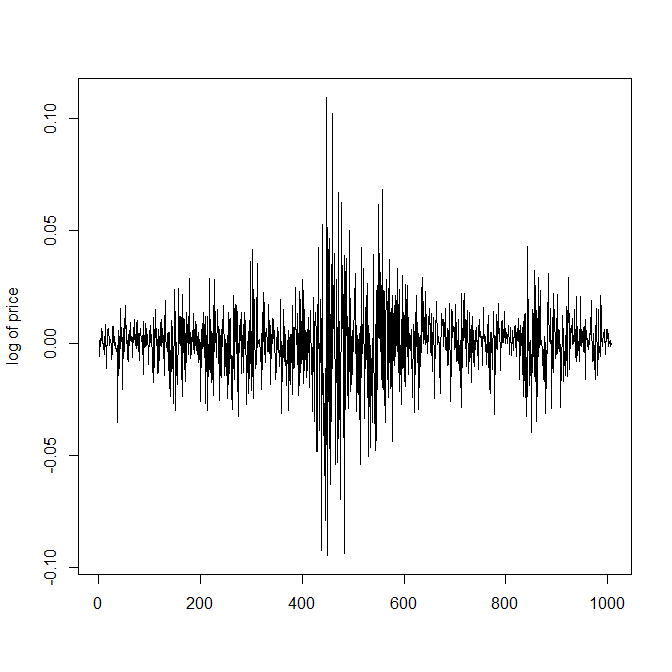
\includegraphics[scale=0.3]{sp}
\caption{Daily change of S$\&$P500 closing price from 2007-2010}\label{9}
\end{figure}

\begin{figure}[H]
\centering
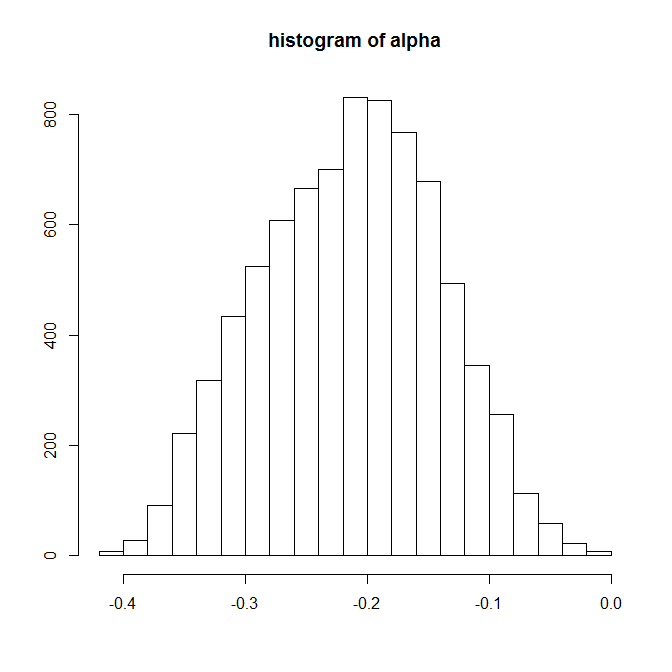
\includegraphics[scale=0.2]{hmrw1halpha}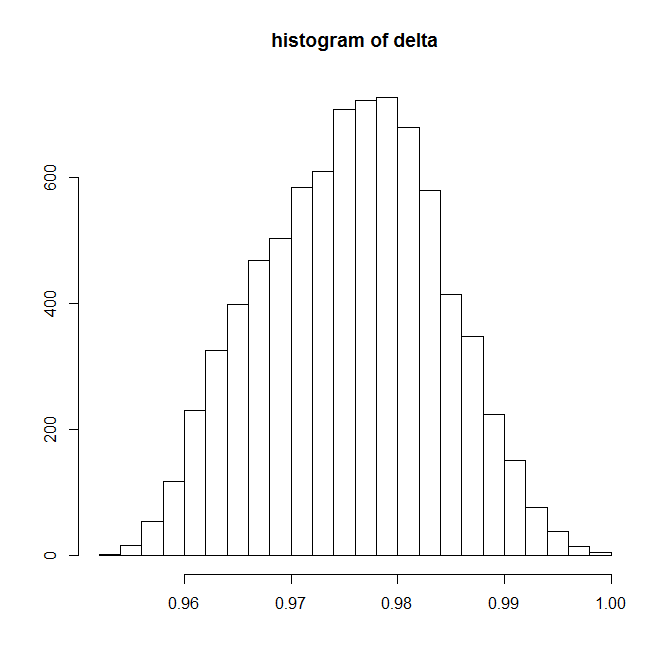
\includegraphics[scale=0.2]{hmrw1hdelta}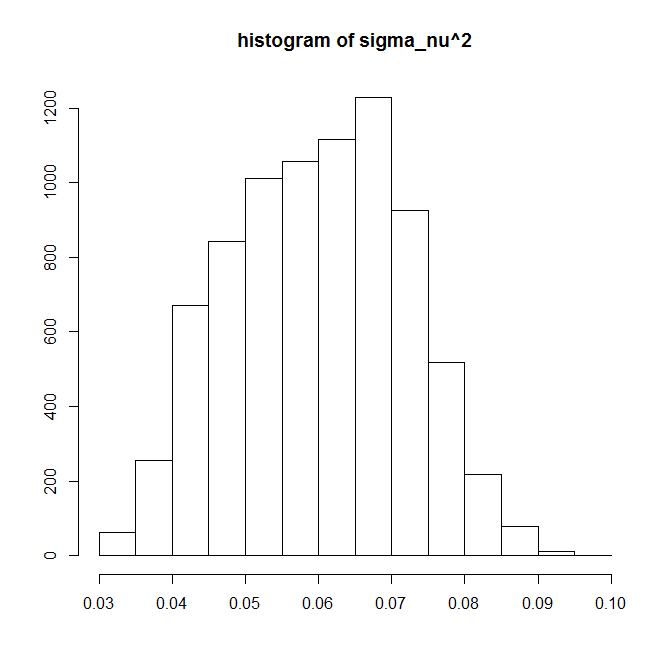
\includegraphics[scale=0.2]{hmrw1hsig}
\caption{Histograms of MH $+$ RW with $e=0.05$}\label{3}
\end{figure}
\begin{figure}[H]
\centering
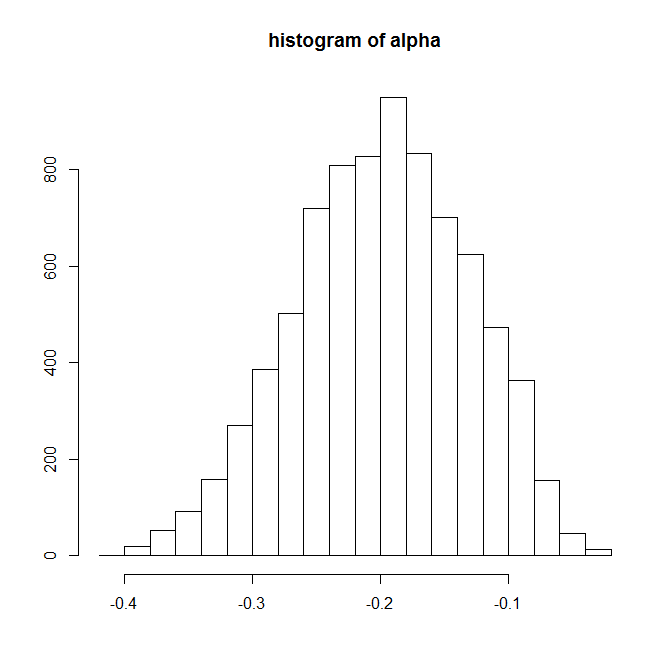
\includegraphics[scale=0.2]{hmrw2halpha}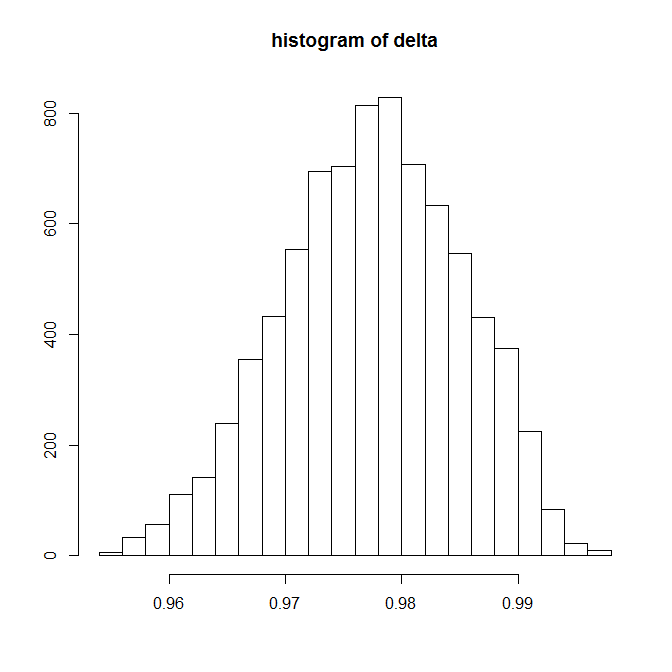
\includegraphics[scale=0.2]{hmrw2hdelta}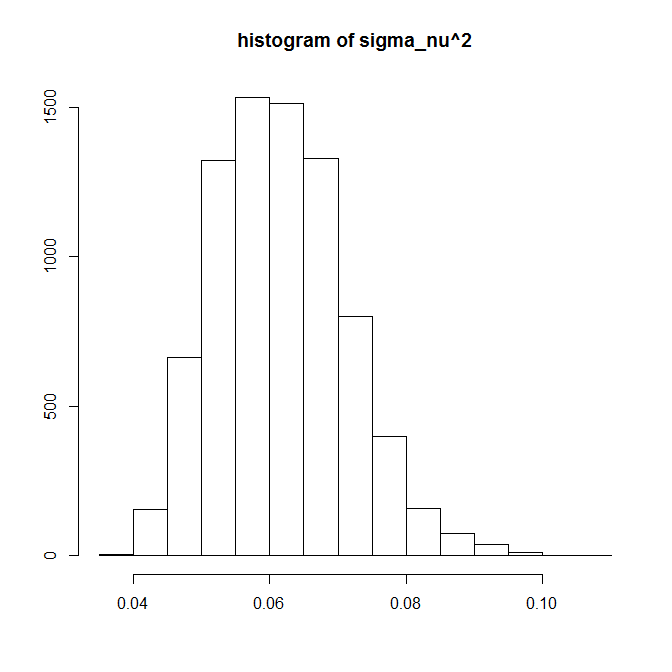
\includegraphics[scale=0.2]{hmrw2hsig}
\caption{Histograms of MH $+$ RW with $e=0.1$}
\end{figure}
\begin{figure}[H]
\centering
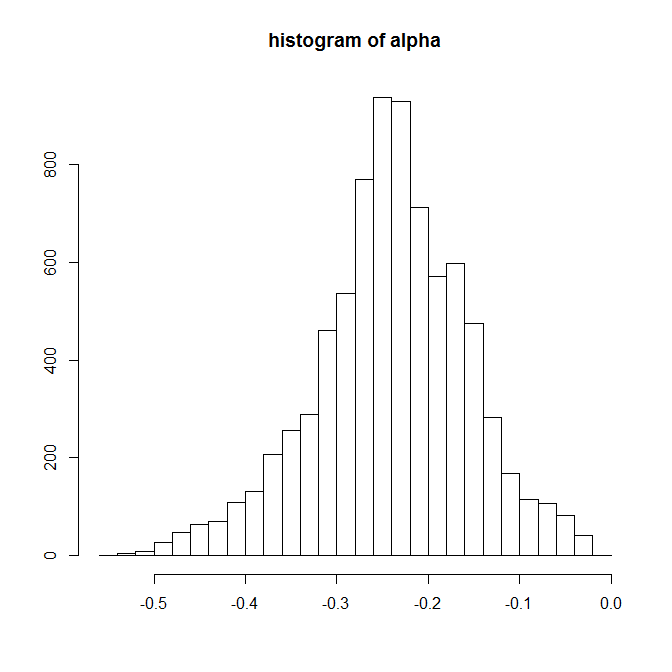
\includegraphics[scale=0.2]{hmrw3halpha}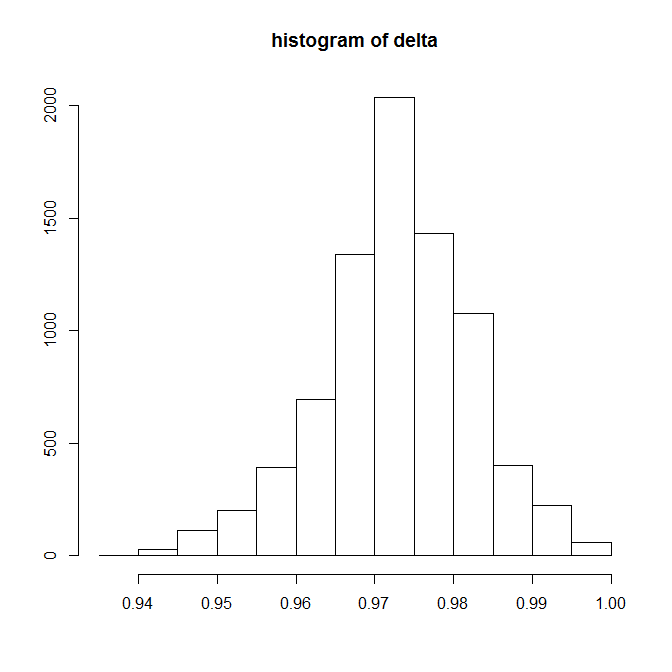
\includegraphics[scale=0.2]{hmrw3hdelta}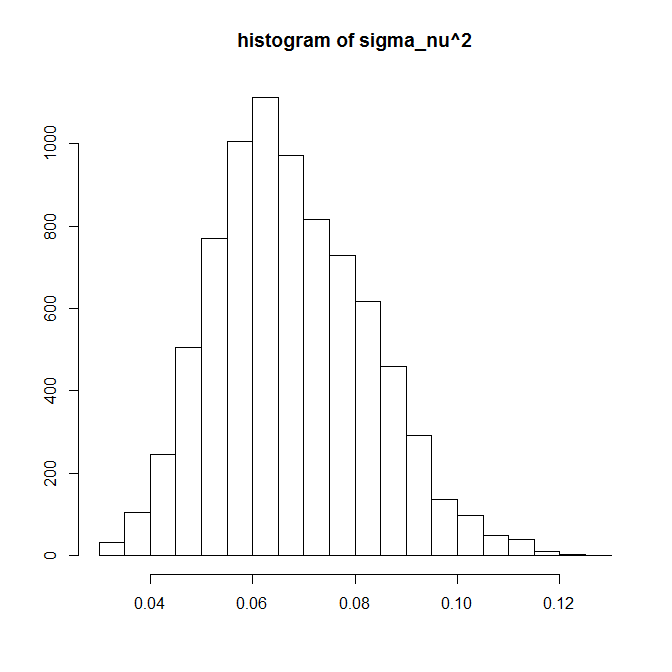
\includegraphics[scale=0.2]{hmrw3hsig}
\caption{Histograms of MH $+$ RW with $e=0.3$}
\end{figure}
\begin{figure}[H]
\centering
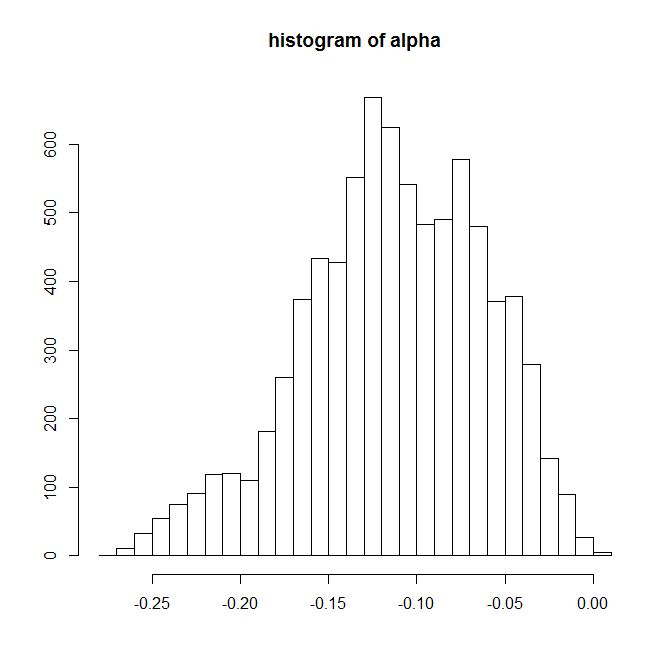
\includegraphics[scale=0.2]{hmrahalpha}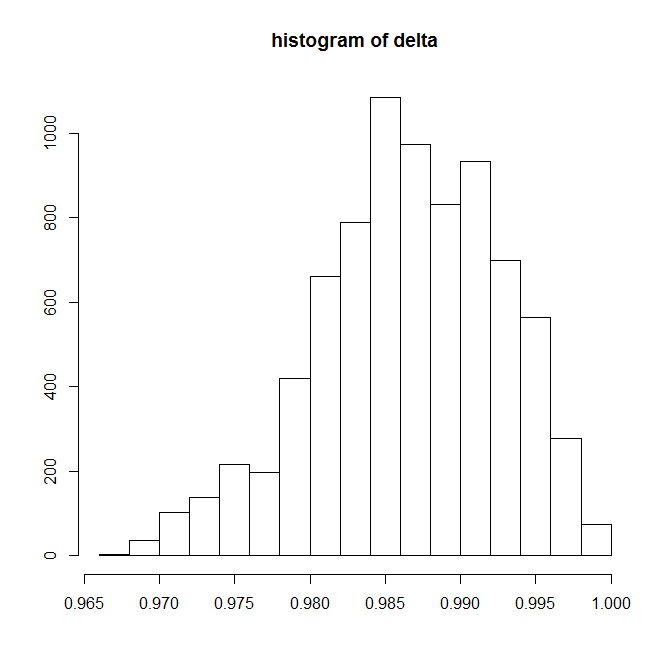
\includegraphics[scale=0.2]{hmrahdelta}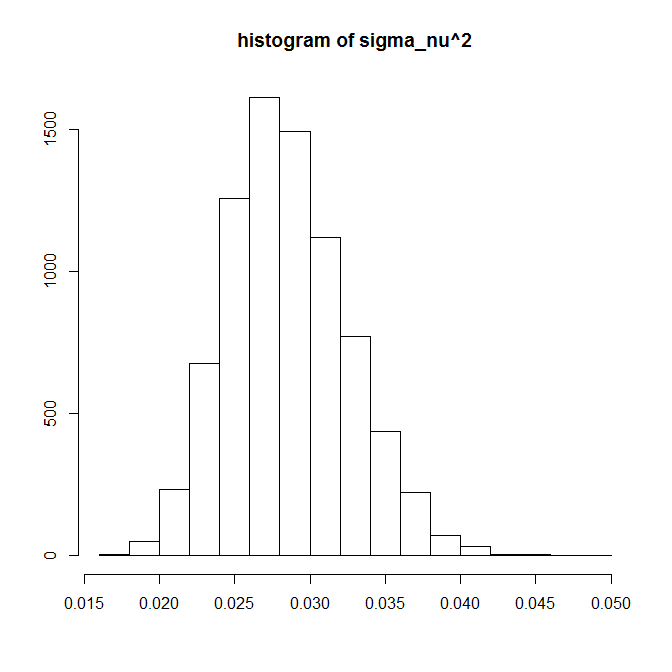
\includegraphics[scale=0.2]{hmrahsig}
\caption{Histograms of MH $+$ RA}
\end{figure}
\begin{figure}[H]
\centering
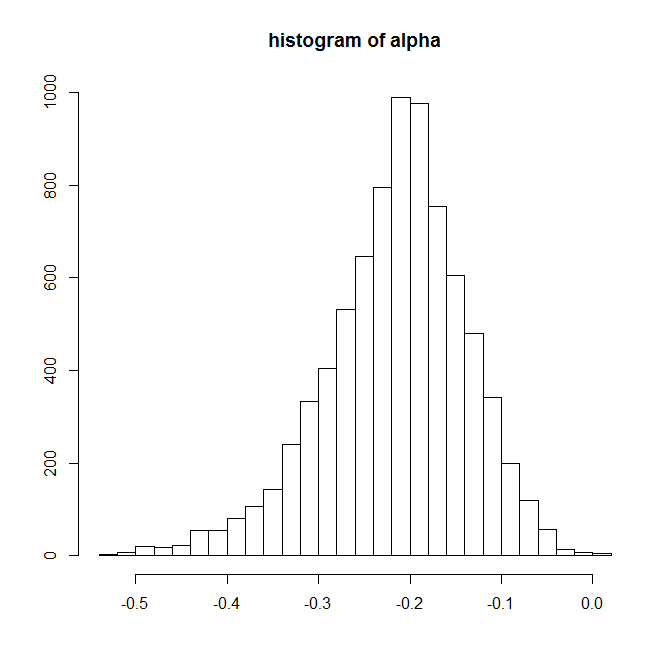
\includegraphics[scale=0.2]{rahalpha}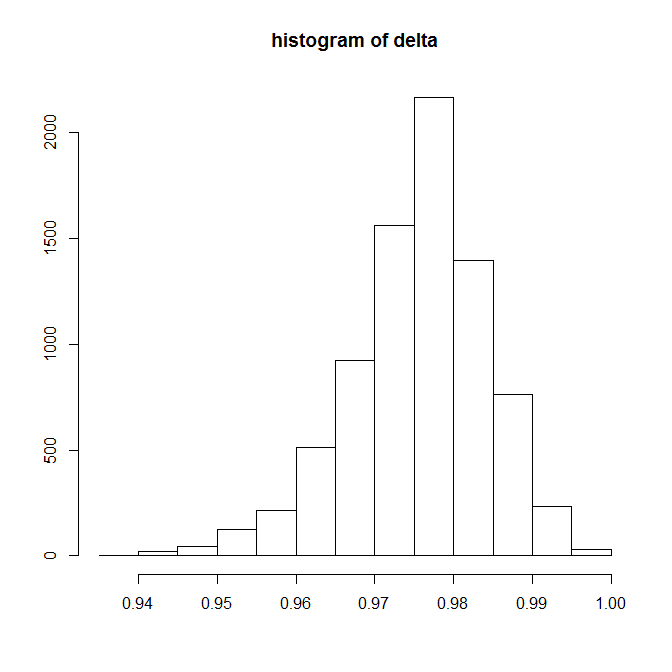
\includegraphics[scale=0.2]{rahdelta}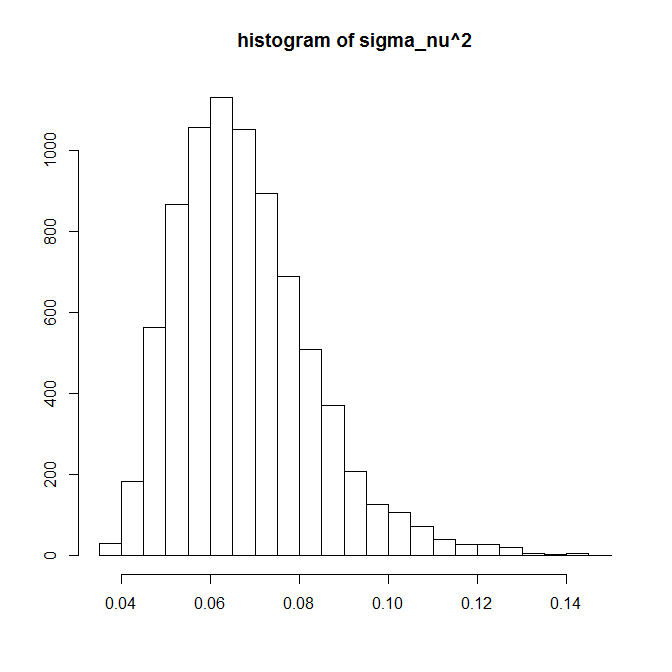
\includegraphics[scale=0.2]{rahsig}
\caption{Histograms of RA}\label{4}
\end{figure}

\begin{figure}[H]
\centering
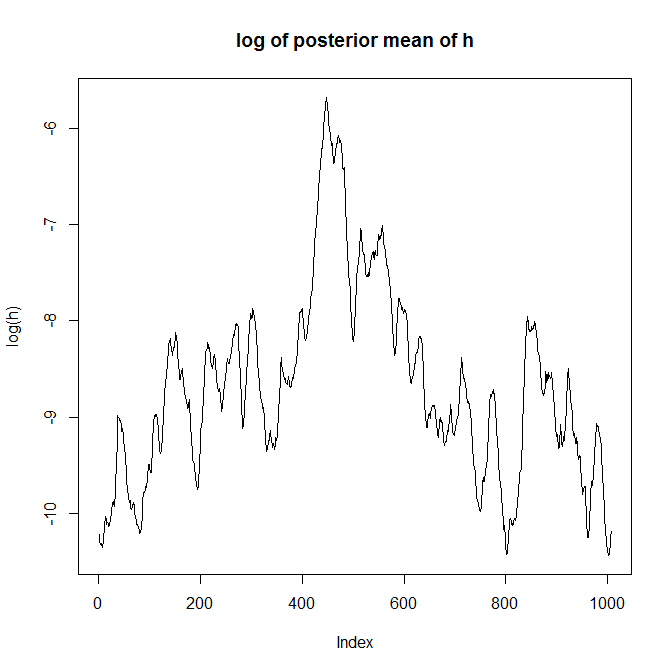
\includegraphics[scale=0.2]{hmrw1h}
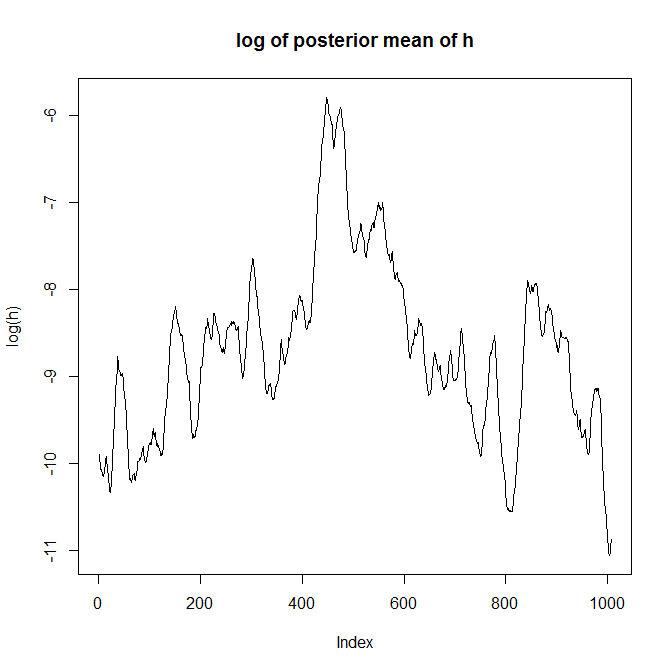
\includegraphics[scale=0.2]{hmrw2h}
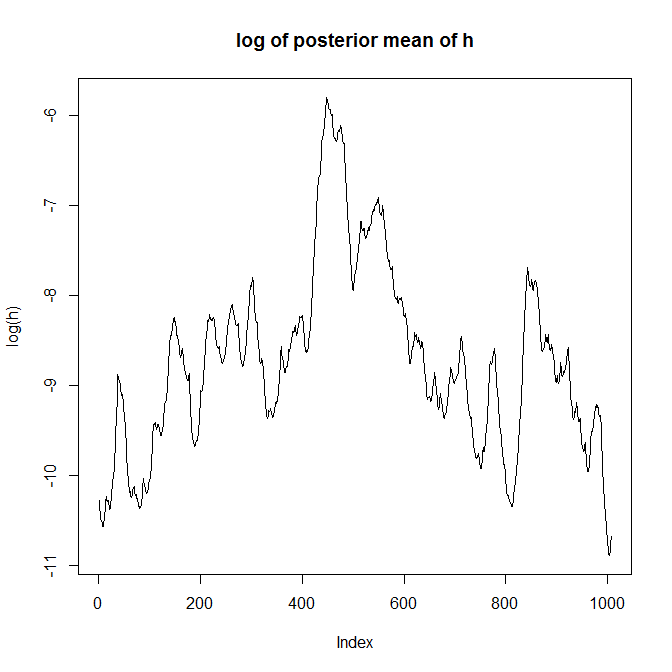
\includegraphics[scale=0.2]{hmrw3h}
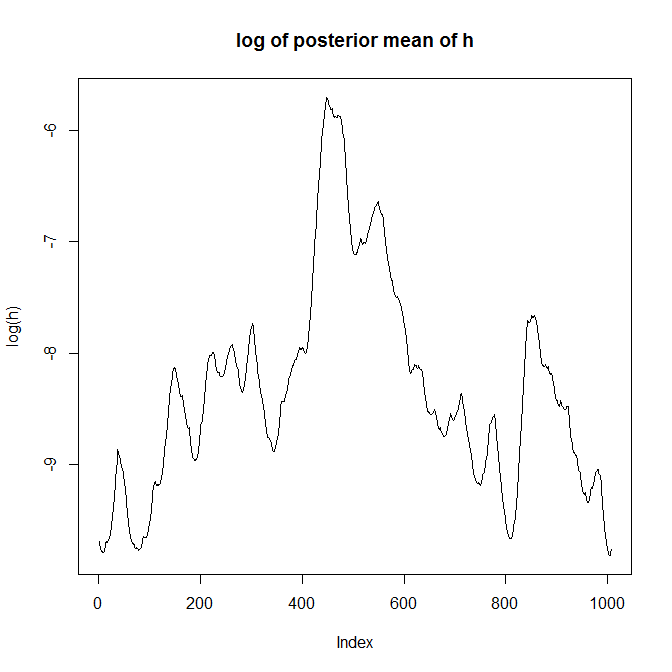
\includegraphics[scale=0.2]{hmrah}
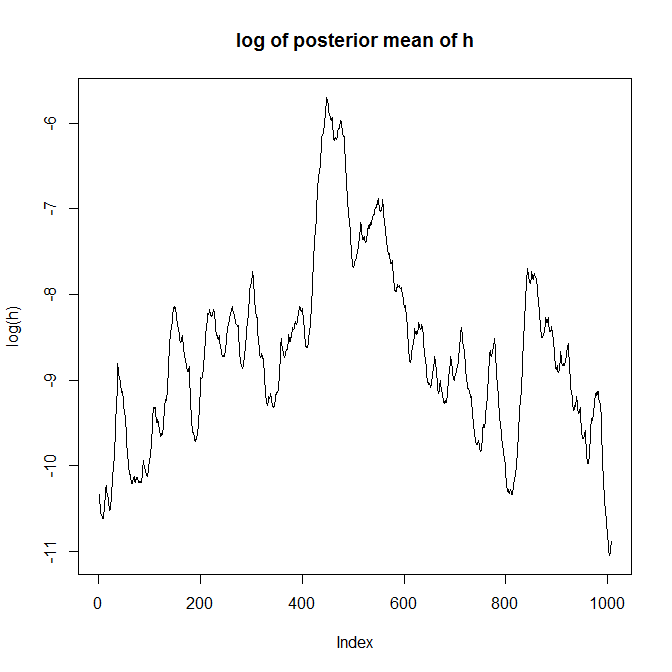
\includegraphics[scale=0.2]{rah}
\caption{Log of mean of $h_t$ of five methods, in the order of appearance in previous tables}\label{5}
\end{figure}

\begin{figure}[H]
\centering
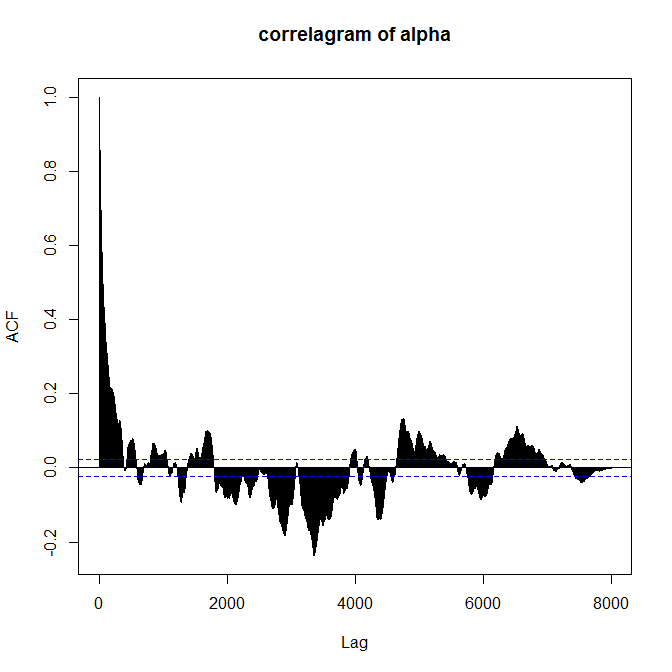
\includegraphics[scale=0.2]{corhmrw1alpha}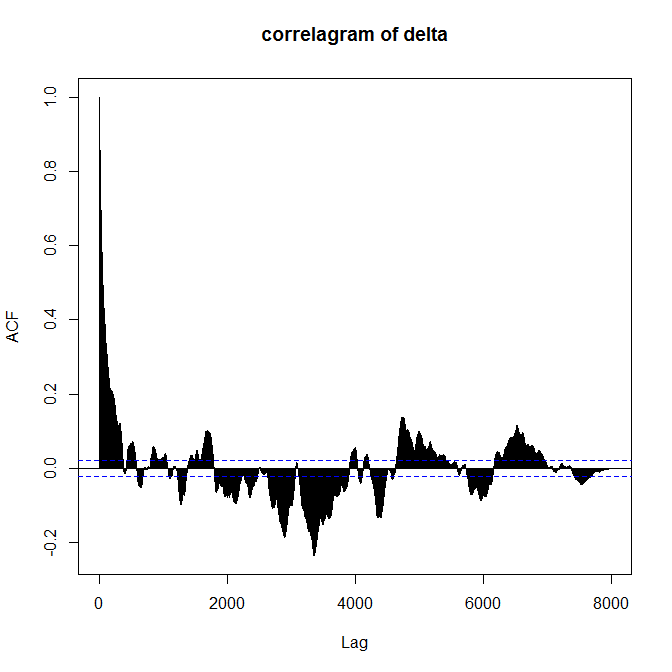
\includegraphics[scale=0.2]{corhmrw1delta}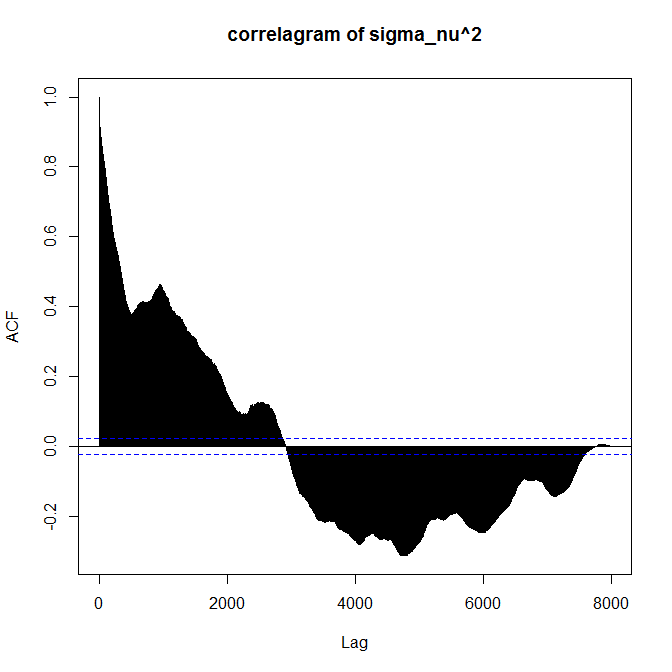
\includegraphics[scale=0.2]{corhmrw1sig}
\caption{Correlagram of MH $+$ RW with $e=0.05$}\label{7}
\end{figure}
\begin{figure}[H]
\centering
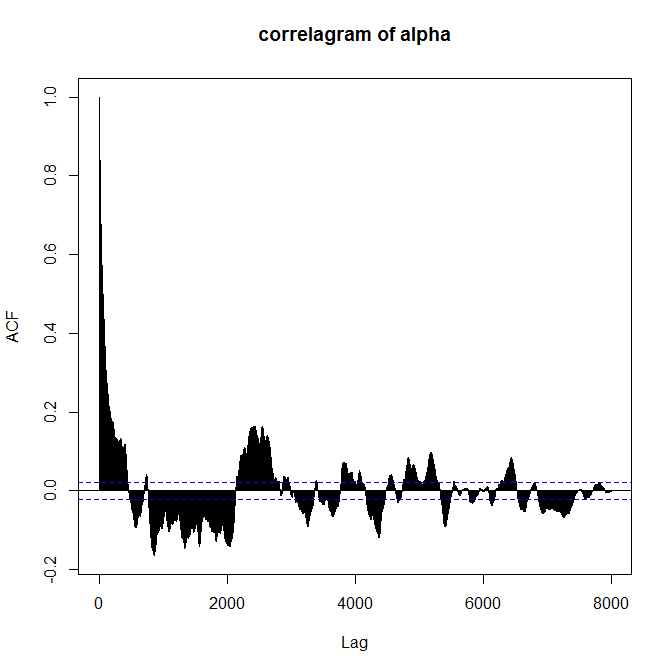
\includegraphics[scale=0.2]{corhmrw2alpha}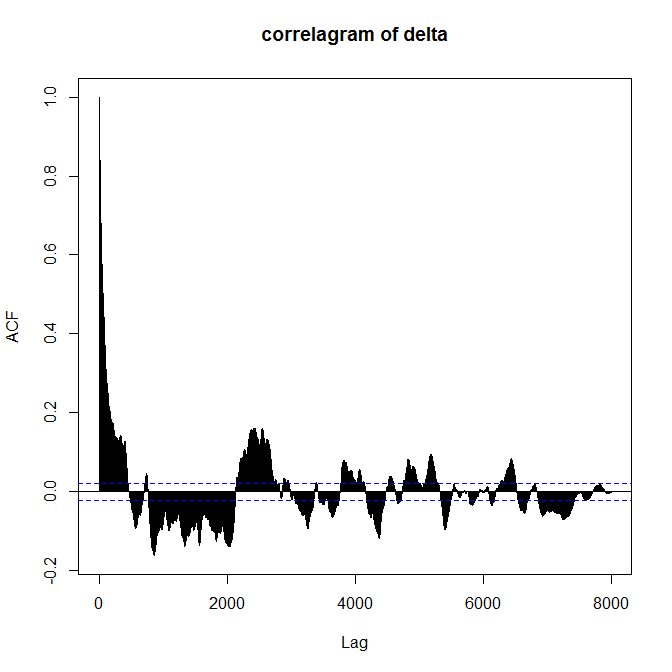
\includegraphics[scale=0.2]{corhmrw2delta}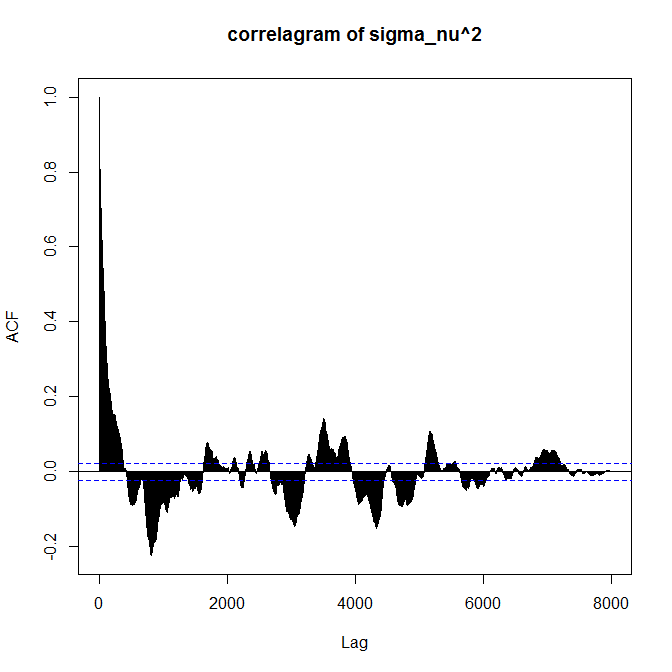
\includegraphics[scale=0.2]{corhmrw2sig}
\caption{Correlagram of MH $+$ RW with $e=0.1$}
\end{figure}
\begin{figure}[H]
\centering
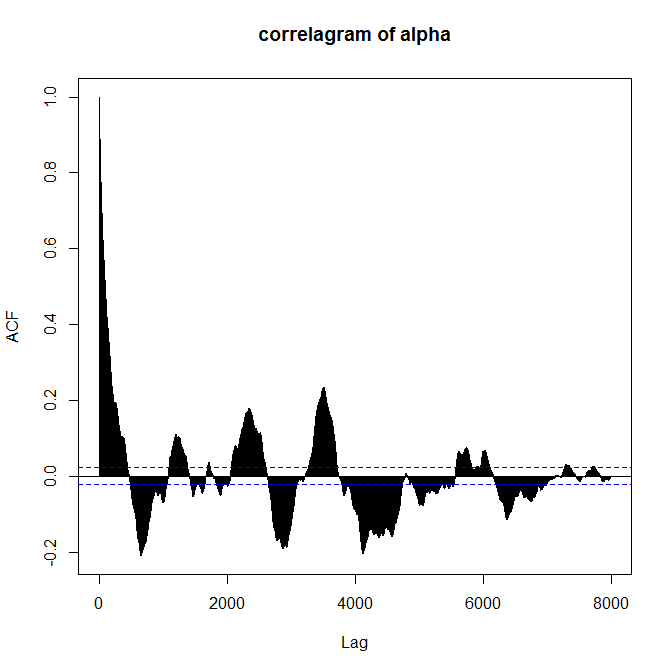
\includegraphics[scale=0.2]{corhmrw3alpha}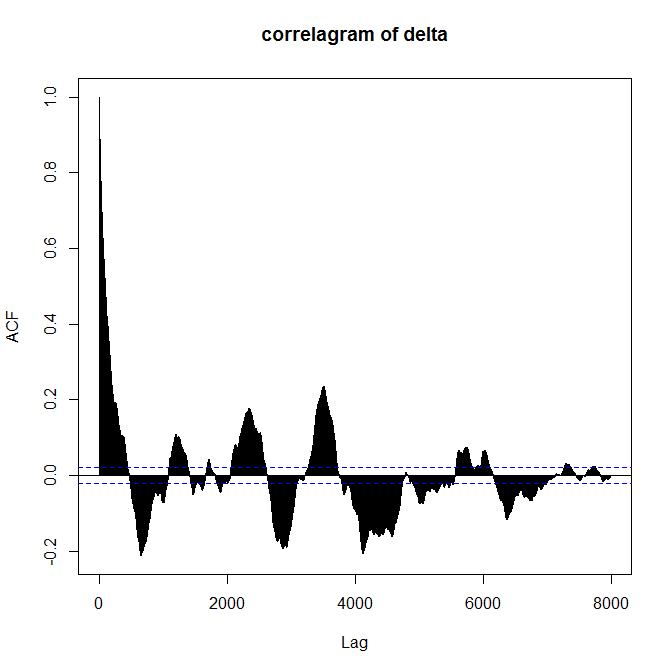
\includegraphics[scale=0.2]{corhmrw3delta}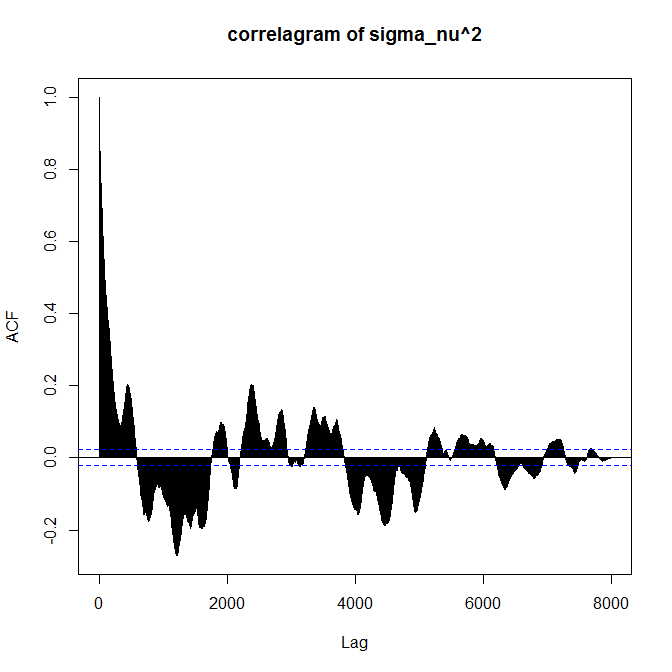
\includegraphics[scale=0.2]{corhmrw3sig}
\caption{Correlagram of MH $+$ RW with $e=0.3$}
\end{figure}
\begin{figure}[H]
\centering
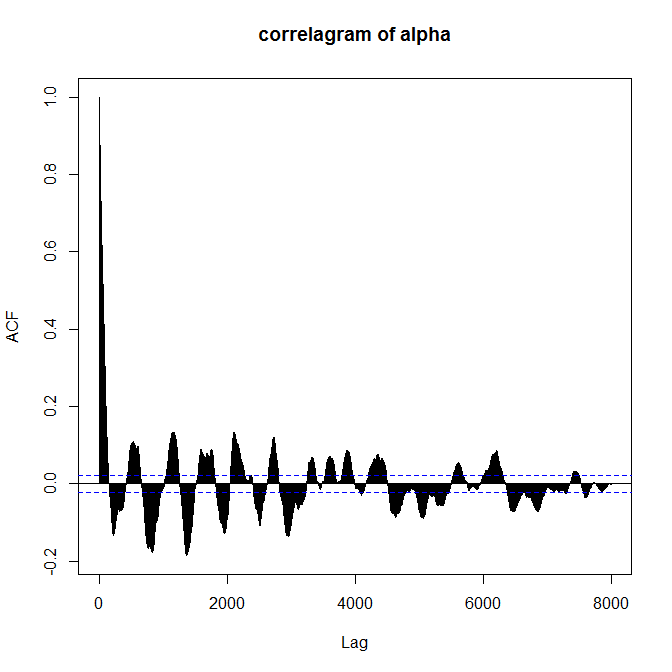
\includegraphics[scale=0.2]{corhmraalpha}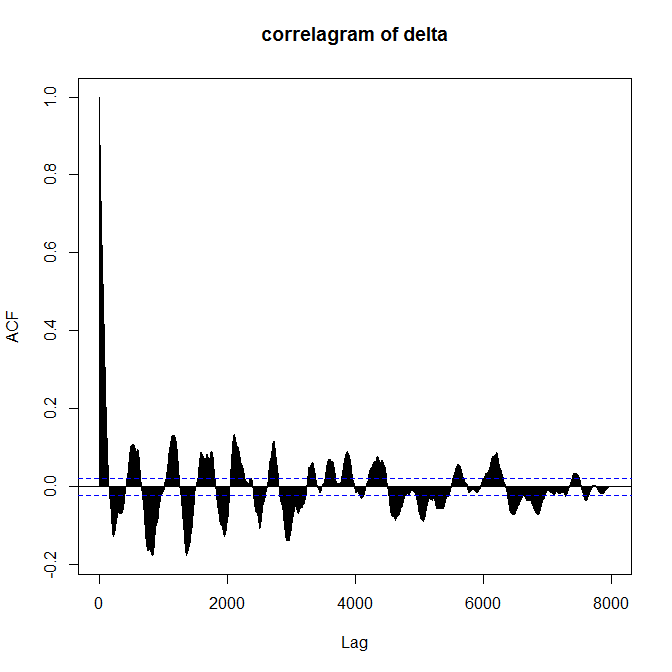
\includegraphics[scale=0.2]{corhmradelta}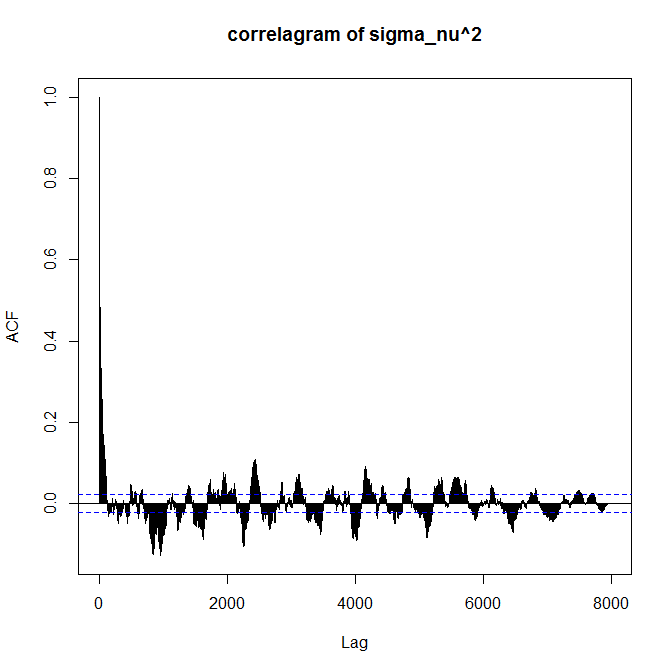
\includegraphics[scale=0.2]{corhmrasig}
\caption{Correlagram of MH $+$ RA}
\end{figure}
\begin{figure}[H]
\centering
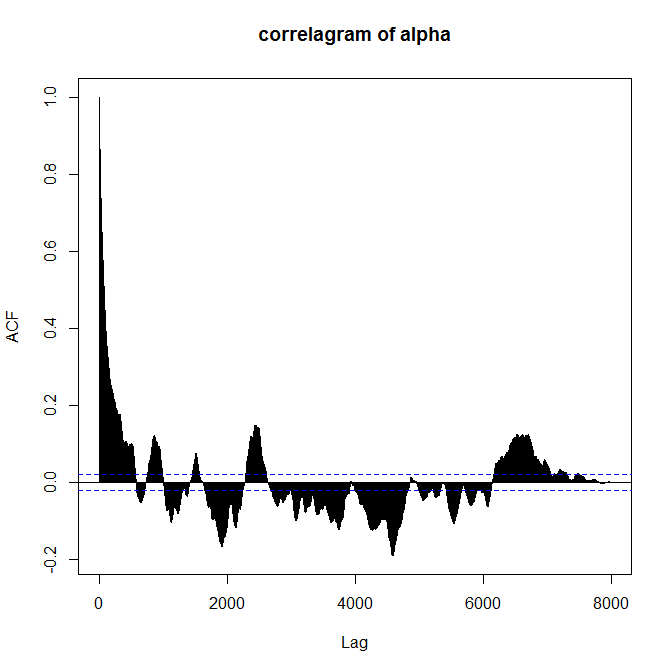
\includegraphics[scale=0.2]{corraalpha}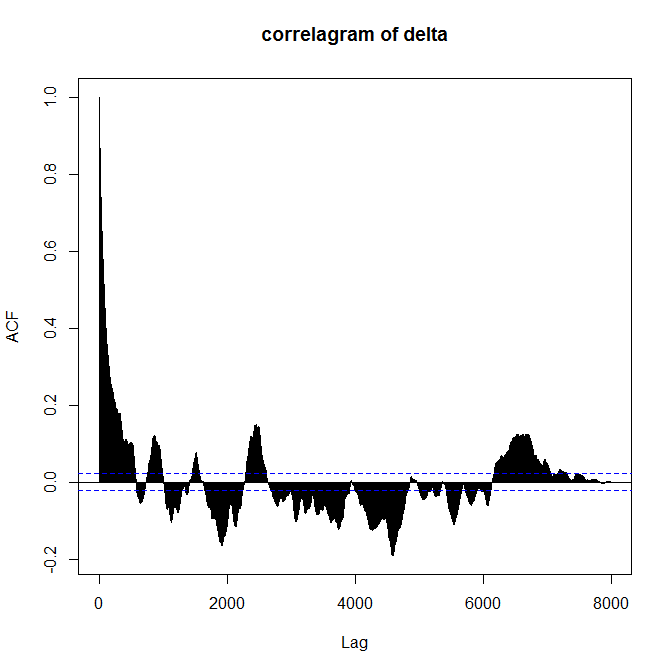
\includegraphics[scale=0.2]{corradelta}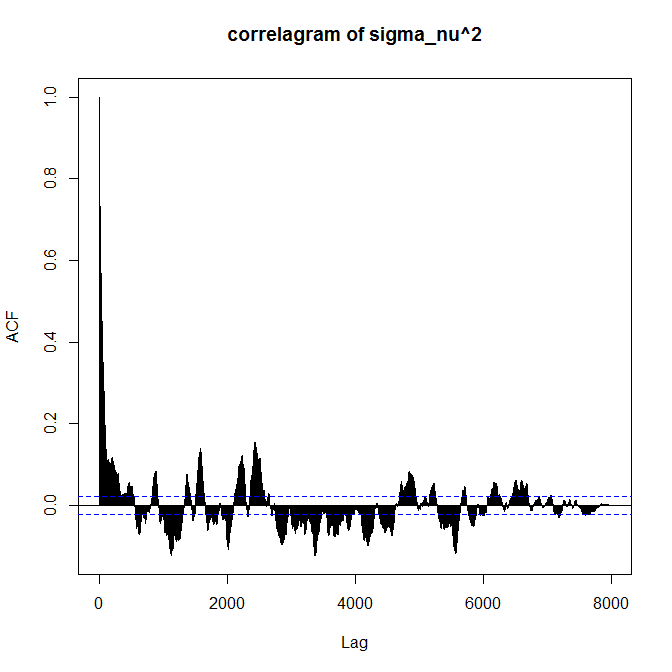
\includegraphics[scale=0.2]{corrasig}
\caption{Correlagram of RA}\label{8}
\end{figure}

\section{Codes}
All codes of this project, along with reference and .png figures appeared in the essay are available in https://github.com/yinanzhu12/MCMC-SV. 

\section{Reference}
\begin{enumerate}
\item
Eric Jacquier, Nicholas G. Polson and Peter E. Rossi, "Bayesian Analysis of Stochastic Volatility Models", Journal of Business $\&$ Economic Statistics, 1994, Vol. 12, No. 4
\item
Eric Jacquier, Nicholas G. Polson and Peter E. Rossi, "Bayesian analysis of stochastic volatility models with fat-tails and correlated errors", Journal of Econometrics, 122(2004) 185-212
\item
John Geweke, "Prior for Macroeconomic Time Series and Their Application", Econometric Theory, Vol. 10, 609-632 (1994a)
\item
John Geweke, "Bayesian Comparison of Econometric Models", working paper, Federal Reserve Bank of
Minneapolis Research Department, (1994b)
\item
Siddhartha Chib and Edward Greenberg, "Understanding the Metropolis-Hastings Algorithm", The American Statistician, Vol. 49, No. 4. (Nov., 1995), pp.327-335
\item
A. Ronald Gallant, Peter E. Rossi, George Tauchen, "Stock Prices and Volume", The Revew of Financial Studies, Vol. 5, No. 2. (1992), pp. 199-242
\item
Sangjoon Kim, Neil Shephard, Siddhartha Chib, "Stochastic Volatility: Likelihood Inference and Comparison with ARCH Model", Review of Economic Studies (1998) 65, 361-393
\end{enumerate}
\end{document}
